\noindent \textbf{Notations}: $\mathbf{X}$表示矩阵,$\vec{x}$表示列向量。

\begin{figure}[h]
    \centering
    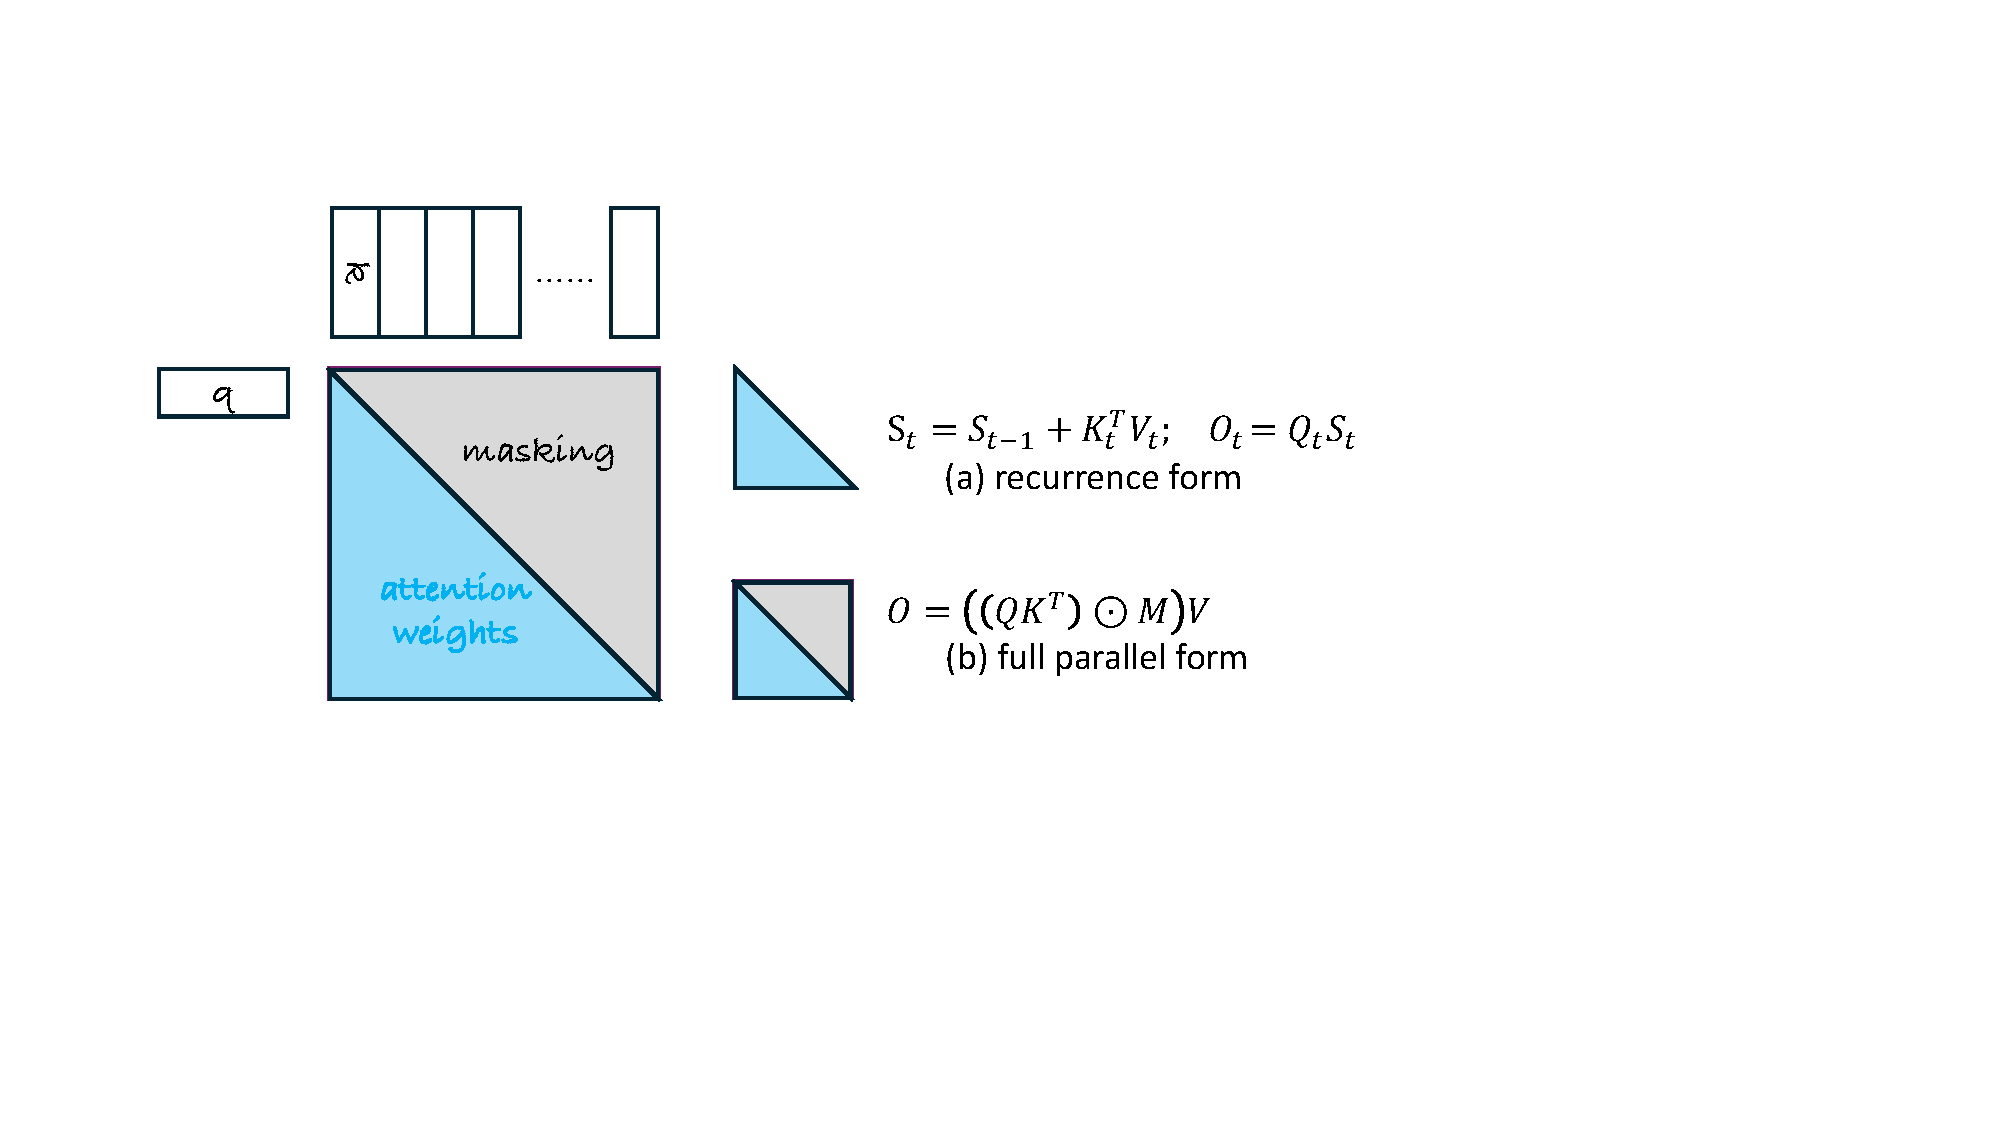
\includegraphics[width=0.6\textwidth]{figures/attention-train.pdf}
    \caption{Transformer的两种计算模式:recurrent form和full parallel form}\label{fig:attention-train}
\end{figure}

训练时我们可以一次性看到全序列,如果token之间不存在数据流依赖,就可以让query token
\footnote{\textbf{\textcolor{red}{这是我们要研究的第一种计算模式。}}}{\colorbox{thistle}{全并行计算}}。

如图\ref{fig:attention-train}所示,上三角部分是冗余计算,通过masking机制消除。
Attention的全并行方式是直接将for循环在空间上全展开。
空间全展开情况下上图上三角部分是冗余计算,需要后续靠点乘一个masking矩阵消除这部分多余计算。

\subsection{Linear Attention\cite{linear-attention-kexue}}

\begin{equation}
O = \text{Attention}(\mathbf{Q},\mathbf{K},\mathbf{V}) = \text{softmax}(\mathbf{Q}\mathbf{K}^T)\mathbf{V} \label{eq:attn1}
\end{equation}

上述公式是多头注意力机制中一个头如何计算的线性代数公式。
其中$\mathbf{Q} \in \mathbb{R}^{L \times d}$,$\mathbf{K}^T \in \mathbb{R}^{d \times L}$,$\mathbf{V} \in \mathbb{R}^{L \times d}$。

目前Transformer模型广泛被用来处理超长序列。假设$E$是隐藏层的维度(一般$E = 512,1024,2048$,在这样的量级)。如果应用了多头注意力机制,会对隐藏层分头$d = \frac{E}{\text{num\_head}}$。
于是$L\gg d$,$\mathbf{P} = \mathbf{Q}\mathbf{K}^T \in \mathbb{R}^{L \times L}$这一步会得到一个非常大的$L^2$大小的中间结果。

仔细分析会发现\textbf{\textcolor{red}{影响attention进一步扩展的是softmax}}。

矩阵乘满足结合律,如果没有softmax,我们可以先计算$\mathbf{S} = \mathbf{K}^T \mathbf{V}$: $[d \times L] [L \times d] = [d \times d]$,得到中间结果大小为$d\times d$,再计算$\mathbf{O} = \mathbf{Q}\mathbf{S}$。由于$d \ll L$,这样的计算过程也会近似地与序列长度呈线性复杂度。

观察attention的sequential计算公式(\textcolor{maroon}{换一种语言来说这里的“sequential计算公式”,也就是把"matrixfied"的线性代数公式展开写成$\sum$求和}):
$$\text{Attention}(\vec{q}_t, \mathbf{K}, \mathbf{V}) = \frac{\sum_{i=0}^{t}\exp \left(\vec{q}_t \vec{k}_i^T\right)\vec{v}_i}{\sum_{i=0}^{t}\exp \left( \vec{q}_t \vec{k}_i^T \right)}$$

我们可以把attention理解为以$\exp \left( \vec{q}_t \vec{k}^T_i \right)$为权值,对$\vec{v}_i$进行加权再求和。于是可以提出一个泛化版的attention:

$$\text{Attention}\left( \vec{q}_i, \mathbf{K}, \mathbf{V} \right) = \frac{\sum_{t=0}^{L}\text{sim} \left(\vec{q}_i, \vec{k}_t \right) \vec{v}_j}{\sum_{t=0}^{L}\text{sim} \left( \vec{q}_i,\vec{k}_t \right)}$$

为了\textcolor{dkgreen}{保持attention的输出结果是一个分布这一关键特性,\textbf{我们要求$\text{sim}(q_t,k_i)\ge 0$}}\footnote{每个分量$\ge 0$是分布的一个最低要求,softmax会得到一个严格的概率分布,求和为0}{。}
基于以上分析,可扩展attention转换为如何设计$\text{sim}\left( \vec{q}_i, \vec{k}_j \right)$。

寻找一个总是大于0的相似度函数可以被转换为许多不同的解决思路,\cite{katharopoulos2020transformers}用了一种简单的思路,给$\vec{q}_t$和$\vec{k}_i$加上限制了值域的激活函数,然后使用内积作为相似性度量。这种方法被解释为“kernel method"。于是我们有如下公式:

$$\vec{o}_t = \frac{\sum_{i=0}^{t}\phi \left( \vec{q}_t \right)\phi \left(\vec{k}_i \right)^T \vec{v}_i}{\sum_{i=0}^{t}\phi \left(\vec{q}_t \right) \phi \left( \vec{k}_i\right)^T} = \frac{\phi \left( \vec{q}_t \right) \sum_{i=0}^{t}\phi \left( \vec{k}_i \right)^T \vec{v}_i}{\phi \left(\vec{q}_t\right) \sum_{i=0}^{t} \phi \left(\vec{k}_i \right)^T}$$

$\mathbf{S}_t \triangleq \sum_{i=0}^{t} \phi \left( \vec{k}_i \right)^T\vec{v}_i$,$\vec{z}_t \triangleq \sum_{i=0}^{t} \phi \left(\vec{k}_i\right)^T$,于是有:

\begin{align}
\mathbf{S}_t &= \mathbf{S}_{t-1} + \phi \left( \vec{k}_t \right)^T\vec{v}_t \nonumber\\
\vec{z}_t &= \vec{z}_{t-1} + \phi \left( \vec{k}_t \right)^T \nonumber \\
\mathbf{O}_t &= \frac{\phi \left( \vec{q}_t \right) \mathbf{S}_t}{\phi \left( \vec{q}_t \right) \vec{z}_t} \label{eq:linear-attn1}
\end{align}

式\eqref{eq:linear-attn1}就是一个泛化版attention框架,不同的工作对$\phi$进行了探索。\textcolor{red}{(1)认为$\phi$取indentity function in practice也够用。(2)有些工作claim 归一化因子$\vec{z}_t$会引起不稳定性,建议可以扔掉$\vec{z}_t$,在输出增加归一化计算},
于是会得到一个如下形式的未归一化的linear attention Transformer:

\begin{align}
\mathbf{S}_t &= \mathbf{S}_{t-1} + \vec{k}_t^T\vec{v}_t \label{eq:linear-attn2}\\
\vec{o}_t &= \vec{q}_t\mathbf{S}_t \nonumber
\end{align}

\textcolor{red}{linear-attention}当作\footnote{\textcolor{red}{这是我们要研究的第二种计算模式。}}{\colorbox{thistle}{RNN式的递归式来}}计算时(图\ref{fig:attention-train}(a)),模型的时间和空间复杂度是序列长度的线性关系,能够节约FLOPS,但是会引入串行性。

如果我们把attention按照下式当作一个矩阵乘来计算(图\ref{fig:attention-train}(b)),模型的时间和空间复杂度是序列长度的平方关系,优点是可以全并行计算。

$$\mathbf{O} = \left( \left(\mathbf{Q}\mathbf{K}^T\right) \odot \textcolor{red}{\mathbf{M}} \right)\mathbf{V}$$

上式$\textcolor{red}{\textbf{M}}$会破坏矩阵乘的结合性,导致如果我们想通过并行方式(时间维度的计算在空间维度全展开),
依然必须先算$\mathbf{Q}\mathbf{K}^T$,再与$\mathbf{V}$相乘,
还是会引起需要存储$L^2$大小的中间结果。

为了让这类模型高效训练,一个折中方案是\footnote{\textcolor{red}{这是我们要研究的第三种计算模式。}}{\colorbox{thistle}{Chunk-wise Block-parallel}} attention。

\begin{align*}
\mathbf{O}_{i+1} &= \mathbf{Q}_{i+1}\mathbf{S}_{i} + \left( \left(\mathbf{Q}_{i+1}\mathbf{K}_{i+1}^T\right) \odot \textcolor{red}{\mathbf{M}} \right)\mathbf{V}_{i+1} \in \mathbb{R} ^{C\times d} \\
\mathbf{S}_0 &= \mathbf{0}
\end{align*}

% \begin{tcolorbox}[colbacktitle=grey!10!white,colback=yellow!3,title={\textbf{\textcolor{grey}{My Take-aways}}}]
% 一个DNN算法是一组任意复杂的线性代数,由于算律满足一定条件\textcolor{red}{(不确定是否能够准确地定义出必要条件?)}会存在两种等价形式:\textit{\textcolor{brown}{空间展开的全并行形式}} vs. \textit{\textcolor{brown}{时间展开的串行方式}},这两种等价形式对系统来说,可能会是一个潜在的调度/决策空间。
% \end{tcolorbox}

\subsection{Linear Attention with Decay}

\colorbox{snow}{\eqref{eq:linear-attn2}显示地表明:\textcolor{red}{\textbf{带线性attention的Transformer,就是一个隐状态是矩阵的RNN}}}。
有许多研究指出,为RNN的state引入decay(衰减)机制,类似于遗忘门的能力,能够有效的改善学习效果。于是引入衰减因子\textcolor{red}{$\gamma$},\eqref{eq:linear-attn2}式改写成如下形式:

\begin{align}
\mathbf{S}_t &= \textcolor{red}{\gamma} \mathbf{S}_{t-1} + \mathbf{K}_t^{T}\mathbf{V}_t
\end{align}

对应的并行形式:

\begin{align*}
\mathbf{O} &= \left( \mathbf{Q}\mathbf{K}^T \odot \mathbf{D}\right)\mathbf{V},
&\mathbf{D} &= \left\{
\begin{aligned}
  &\gamma^{n-m}, &n \ge m \\
  &0, &n < m
\end{aligned}
\right.
\end{align*}

\subsection{典型代表}

\subsubsection{RetNet\cite{sun2023retentive}}

RNN模型相关研究表明:遗忘门对改善学习效果有着重要作用。

在DNN模型学习效果方面,RetNet的一个设计要素是:在recurrent计算对状态的更新过程中,
引入一个显示的衰减(decay term)能够极大的改善学习效果,一些情况下甚至可以超过标准的softmax Transformer。

\begin{displayquote}
adding a global decay term to the additive RNN update rule greatly improves performance, sometimes outperforming standard Transformers with softmax attention when trained at scale.\cite{yang2023gated}
\end{displayquote}

\subsubsection{GAU\cite{hua2022transformer}}

\subsubsection{GLA\cite{yang2023gated}}
